\section{Algorithm}
\subsection{U-Net}
There are mainly 3 tricks to train a U-Net, namely overlap-tile strategy, data augmentation and weighted loss.
\subsubsection{Overlap-tile strategy}
This strategy allows the seamless segmentation of arbitrarily large images. See Figure~\ref{fig:overlap}
To predict the pixels in the border region
of the image, the missing context is extrapolated by mirroring the input image.
This tiling strategy is important to apply the network to large images, since
otherwise the resolution would be limited by the GPU memory.
\begin{figure}[!htpb]
    \centering
    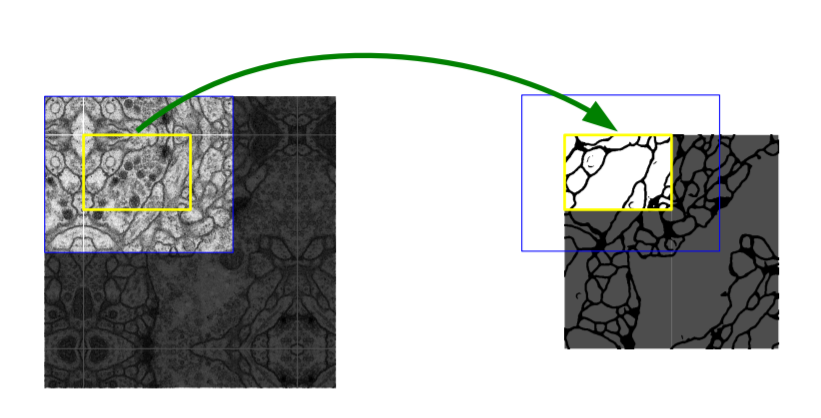
\includegraphics[scale=0.3]{figuras/overlap-tile.PNG}
    \caption{ Overlap-tile strategy for seamless segmentation of arbitrary large images. Prediction of the segmentation in
    the yellow area, requires image data within the blue area as input. Missing input data
    is extrapolated by mirroring}
    \label{fig:overlap}
    \end{figure}
\subsubsection{Data augmentation}
As for our tasks there is very little training data available, we use excessive
data augmentation by applying elastic deformations to the available training images. This allows the network to learn invariance to such deformations, without
the need to see these transformations in the annotated image corpus. This is
particularly important in biomedical segmentation, since deformation used to
be the most common variation in tissue and realistic deformations can be simulated efficiently. 

In case of microscopical images we primarily need shift and rotation invariance as well as
robustness to deformations and gray value variations. Especially random elastic deformations of the training samples seem to be the key concept to train
a segmentation network with very few annotated images. We generate smooth
deformations using random displacement vectors on a coarse 3 by 3 grid. The
displacements are sampled from a Gaussian distribution with 10 pixels standard
deviation. Per-pixel displacements are then computed using bicubic interpolation. Drop-out layers at the end of the contracting path perform further implicit
data augmentation.
\subsubsection{Weighted loss}
We pre-compute the weight map for each ground truth segmentation to compensate the different frequency of pixels from a certain class in the training
data set, and to force the network to learn the small separation borders that we
introduce between touching cells. 

The separation border is computed using morphological operations. The
weight map is then computed as
$$
w(\mathbf{x})=w_c(\mathbf{x})+w_0\cdot \exp \left(- \frac{(d_1(\mathbf{x})-d_2(\mathbf{x}))^2}{2\sigma^2}\right)
$$
where $w_c: \Omega \rightarrow R$ is the weight map to balance the class frequencies, $d_1: \Omega \rightarrow R$ denotes the distance to the border of the nearest cell and $d_2: \Omega \rightarrow R$ the distance
to the border of the second nearest cell. 